\documentclass[a4paper]{article}

\usepackage[czech]{babel}
\usepackage[utf8]{inputenc}
\usepackage[T1]{fontenc}
\usepackage{outlines}
\usepackage[hidelinks]{hyperref}

\usepackage[left=1.5cm, text={18cm, 26cm}, top=1.8cm]{geometry}

\usepackage{graphicx}
\usepackage{float}
\usepackage[usenames, dvipsnames]{xcolor}

\hypersetup {
    unicode = true,
    pdfauthor = {Josef Škorpík, Martin Pech},
    pdftitle = {Simulační studie},
    pdfsubject = {IMS},
    pdfkeywords = {IMS Projekt, balistika, ShKH vz. 77 Dana},
    % pdfproducer = {},
    % pdfcreator = {pdfTeX}
}            

\newcommand{\logo} {
    
\includegraphics[scale=0.8, keepaspectratio]{fig/logo.pdf}
}

\renewcommand*{\ttdefault}{lmtt}

\pdfminorversion=7


\begin{document}

    \begin{titlepage}
        \begin{center}
            \logo
            \\\vspace{\stretch{0.382}}
            {\Huge Simulační studie}\\\medskip
            {\LARGE Implementace abstraktního modelu autobusové linky}\\\medskip
            {\large	Hromadná osobní přeprava}
            \vspace{\stretch{0.618}}
        \end{center}
        {\Large \today \hfill
        \begin{tabular}{l l}
            \textbf{Martin Pech} & \textbf{(\texttt{xpechm00})} \\
            Josef Škorpík & (\texttt{xskorp04})
        \end{tabular}}
    \end{titlepage}

    \newpage

	\section{Úvod}
    \label{sec:intro}

    Tématem projektu je implementace abstraktního modelu~\cite[snímek 10]{IMS_slides} autobusové linky.
    Projekt vznikl jako zápočtová práce do předmětu Modelování a simulace. Chování modelu bylo demonstrováno na základě existující Jihomoravské autobusové linky číslo 501. Tento model si klade za cíl najít optimální počet autobusů, které je potřeba rezerovovat pro danou linku tak, aby nedocházelo k dlouhému čekání a najít optimální jízdní řád na základě zadaných parametrů o hustotě provozu. Optimální počet autobusů i jízdní řád hledáme podle spokojenosti cestujících, která je ovlivněna tím, jestli přijedou do cílové stanice včas, nebo se zpožděním. Jelikož je tento simulační model~\cite[snímek 44]{IMS_slides} zacílen pouze na tyto konkrétní cíle, uvažuje pouze takové jevy, které přímo ovlivňují chování modelu. Tyto jevy jsou popsány v kapitole ~\ref{subsec:conceptual_model_description}.

        \subsection{Autoři a~původ faktů}
        \label{subsec:authors}

            Na implementaci projektu a~tvorbě technické zprávy spolupracovali studenti Fakulty informačních technologií Vysokého učení technického v~Brně, Martin Pech a~Josef Škorpík.
            
            Údaje o počtu zastávek, průměrné době mezi zastávkami a intervalech mezi výjezdy autobusů, které byly použity pro výchozí nastavení modelu vycházejí z veřejně přístupných jízdních řádů uveřejněných na webu Integrovaného dopravního systému Jihomoravského kraje\cite{Jizdni_rad}. 
            Pravděpodobnost výskytu dopravní nehody byla spočítána na základě veřejně dostupných statistik pro rok 2020, které každoročně uveřejňuje Policie České republiky a podle informací poskytnutých Ministerstevm dopravy České republiky k říjnu roku 2020\cite{Accident_statistics}. Pro výpočet této hodnoty bylo uvažováno následujících faktů:
            \begin{outline}
            	\1 Počet platných řidičských průkazů: \textbf{6 002 348}
            	\1 Počet dopravních nehod: \textbf{94 797}
            	\2 Z toho počet dopravních nehod s jedoucím nekolejovým vozidlem: \textbf{28 333}
            \end{outline}
            
            Pro výpočet cílové pravděpodobnosti bylo dále uvažováno, že se žádná osoba neúčastnila nehody vícekrát. Výsledná pravděpodobnost se tedy rovná přibližně \textbf{1 : 212}, což odpovídá cca \textbf{0.0047\%}.
            
            Výchozí údaje o dopravní zácpě byly zjištěny experimentálně. Vybrali jsme si linku č. 501, jelikož s ní má jeden z~řešitelů (Martin Pech) mnoho zkušeností. Od 10.09.2023, kdy jsme projekt začali řešit, jel celkově touto linkou 60 krát tam a 60 krát zpět. Tudíž za tři měsíce s ní jel celkově 120x. Z toho 80x jel v čas, který považujeme za dopravní špičku a 40x v čase, který nepovažujeme za dopravní špičku. Data ohledně dopravní zácpy jsme tedy získali experimentálně. Pokud se nejedná o čas dopravní špičky, průměrně se autobus dostal do dopravní zácpy v 5\% a to způsobilo zpoždění průměrně 5 minut. Pokud se autobus do dopravní zácpy nedostal, došlo maximálně k tak malému zpoždění, které zanedbáváme (zanedbáváme zpoždění, které nepřesáhne 2 minuty). \\
            Určení pravděpodobnosti zácpy ve špičce bylo spočítáno na základě pokusu, tedy skutečného ježdění danou linkou. V době kdy ještě neexistoval vylukový jízdní řád, nastávala dopravní zácpa vždy na jedná konkrétní zastávce. Jelikož se jednalo o jednu z 7, pravděpodobnost výskytu tohoto jevu by se dala popsat jako 1/7. Průměrná doba v této zácpy se pohybuje okolo 17 minut.\\
            Dále bylo třeba zjistit, kolik bude průměrně cestujících na jednotlivých autobusových zastávkách. Vycházíme ze statistik\cite{Pocet_cestujicich}, uvedených na portálu wikipedie.org. V roce 2022 provozoval Dopravní podnik města Brna 328 autobusů určených pro městskou osobní dopravu. Tyto autobusy v roce 2022 přepravily 111.7 milionů cestujících. \\
            Z toho jsme spočítali, že jeden autobus převeze průměrně 39 lidí za hodinu. Naše trasa linky č. 501 trvá 21 minut, za které tedy autobus převeze průměrně 13 lidí. Jelikož je na lince 7 zastávek, počítáme s tím, že průměrně budou na každé zastávce 2 lidi. Tyto statistiky vychází z celoročních dat, tudíž zde počítáme jak spoje v dopravní špičce, tak např. noční spoje, ve kterých bude nejspíše méně lidí. Jedná se tedy o čistý průměr, ale můžeme předpokládat, že pokud budeme uvažovat čas dopravní špičky, počet cestujících bude větší.

        \subsection{Validace výstupů}
        \label{subsec:validation}
        V této práci provedeme několik experimentů (popsané v kapitole \ref{sec:simulation}) a výsledky těchto experimentů budeme validovat tak, že porovnáme data, které z experimentu budou vyplývat, s daty, které jsou obsaženy v jízdním řádě. Pokud nasimulujeme existující linku hromadné dopravy a náš model usoudí, že cestující jsou při používání této linky spokojeni, pak není třeba jízdní řád dané linky měnit. Pokud by cestující byli nespokojeni, je třeba experimentovat s proměnnýma (např. s počtem autobusů, které jezdí na dané lince), abychom byli schopni optimalizovat jízdní řád a najít ten ideální.
	
\newpage
    \section{Rozbor tématu a~použitých metod/technologií}
    \label{sec:methods}
        Autobusová linka, kterou jsme se rozhodli modelovat, je linka č.~501. Popis této linky mimo dopravní špičku odpovídá defaultnímu nastavení naší simulace. Autobusy jezdí z Ústředního hřbitova do Ořechova. Linka má 7 autobusových zastávek a celková doba jízdy autobusu po této lince (bez zpoždění) je 21 minut. Naše simulace běží v čase, který odpovídá sekundám, tudíž to odpovídá 1260 sekundám. Šance na to, že autobus havaruje je 0.0047\%. V takovém případě vyšleme náhradní autobus, který převezme všechny cestující z havarovaného autobusu a pokračuje dál na lince. Počítáme s tím, že průměrně na každé zastávce budou 2 lidé. Obecně ale platí, že se cestující generují rovnoměrným rozložením, daným intervalem <0, x>, kde x si můžeme nastavit přepínačem \texttt{-i}. Stejně pak pracujeme s počtem cestujících, kteří vysednou na zastávce. Počet cestujících, kteří vysedají na zastávce je dán rovnoměrným rozložením s intervalem <0,y>, kde y je možné si nastavit parametrem \texttt{-o}. Ze statistik (uvedeno v \ref{subsec:authors}) vyplývá, že průměrně do autobusu na zastávce vstoupí 2 lide. Počítáme i s tím, že průměrně 2 lidé z autobusu odejdou. Takže defaultní hodnota pro proměnné x,y je~4. Průměrně naložení a vyložení cestujících trvá 90s (1.5 minuty). Průměrný čas mezi jednotlivými zastávkami na této lince je 78 sekund (1.3 minuty). Nový autobus vyjíždí na linku každých 675 sekund, tedy každých 11.25 minut. Celkem na tuto linku máme 2 autobusy a každý z nich má kapacitu 75 míst. Budeme tedy zkoumat, jaký je optimální počet autobusů pro danou linku. Rozhodování toho, co je optimální, stojí hlavně na spokojenosti cestujících. Pokud cestující dojedou včas, jsou spokojení. Pokud se autobus, ve kterém jedou, dostane do havárie, nebo se dostanou do zácpy a přijedou pozdě, ovlivní to spokojenost v negativním smyslu. Náš nástroj také sleduje využitelnost autobusů. Pokud si na linku rezervujeme 8 autobusů, ale 5 z nich nevyužijeme, je to ekonomicky neúnosné.\\
        Důležité je zmínit, že náš nástroj sice defaultně simuluje autobusovou linku č. 501 mimo dopravní špičku, ale všechny proměnné můžeme nastavit pomocí parametrů (popsáno v \ref{subsec:start}). Tudíž je použitelný na jakoukoliv linku hromadné dopravy , u které bychom chtěli zoptimalizovat jízdní řád, nebo se ujistit, že jízdní řád je navržen správně.
        \subsection{Popis použitých postupů}
        \label{subsec:methods}

            K vytvoření základní koncepce projektu jsme využili deklarativních modelů~\cite[snímek 49]{IMS_slides}, konkrétně Petriho sítě~\cite[snímek 123]{IMS_slides} vyobrazené níže.
            Pomocí Petriho sítí byla vytvořena obslužná linka simulující chování linky hromadné dopravy. Pro implementaci jsme si zvolili jazyk C++, jelikož je velmi dobře využitelný v případech, kdy je nutný vysoký výkon. Proto je to ideální volba právě pro tvorbu simulací, které mohou být výpočetně náročné. Pro účely modelování využíváme knihovnu SIMLIB \footnote{\url{https://www.fit.vutbr.cz/~peringer/SIMLIB/}} ve verzi 3.09. Pro sestavení projektu jsme použili GNU Make \footnote{\url{https://www.gnu.org/software/make/}}. Nástroj i knihovna jsou volně dostupné a jsou distribuovány pod svobodnou licencí softwaru.
            

        \subsection{Popis původu použitých metod/technologií}
        \label{subsec:techology}

            Jak již bylo zmíněno, pro implementaci byl použit jazyk C++ v~kombinaci s~knihovnou SIMLIB ve verzi 3.09. S~pomocí tohoto jazyka
            bylo přistupováno k~rozhraní knihovny SIMLIB, pomocí kterého byly vytvořeny předpisy pro všechny komponenty potřebné k~simulaci.
            Pro sestavení programu byl použit GNU Make.

    \section{Koncepce modelu}
    \label{sec:concept}

        Konceptuální model~\cite[snímek 48]{IMS_slides} je koncipován jako systém hromadné obsluhy~\cite[snímek 136]{IMS_slides}.
        Pracuje se dvěmi obslužnými linkami. První je autobus s defaultní kapacitou 75, a druhá je autobusová zastávka. Simlujeme sice autobusovou linku s číslem 501, ale model se dá použít na modelování libovolné linky hromadné dopravy. Takže se náš model neomezuje na počet autobusových zastávek linky 501, či na předem daný počet autobusů. Další činitelé v našem modelu jsou dopravní zácpy a havárie. Pokud by autobus havaroval, bude vyslán další autobus, který dojede na místo havárie, převezme cestující z havarovaného autobusu a pokračuje dál předem danou trasou.

        \subsection{Popis konceptuálního modelu}
        \label{subsec:conceptual_model_description}
            Do modelu vstupují jednotlivé autobusy v intervalu daným tím, jakou linku modelujeme (lze nastavit parametrem~\texttt{-s}).
            V čas výjezdu autobus vyjíždí na první autobusovou zastávku. Na zastávce nabírá cestující. Mohou nastat dvě komplikace. Autobus může havarovat, tudíž systém vyšle nový autobus na místo havárie a převezme cestující. Poté pokračuje v dané lince. Nebo se autobus může dostat do dopravní zácpy. Výstupem modelu je spokojenost cestujících. Spokojenost je ovlivněna časem příjezdu do cílové destinace. Pokud cestující přijede bez komplikací a včas, dá se říct, že se službou dané linky byl spokojený. Pokud se dostane do havárky nebo dopravní zácpy, autobus přijede se zpožděním a můžeme očekávat, že cestující nebude se službou spokojen.
            
\newpage
        \subsection{Forma konceptuálního modelu}
        \label{subsec:conceptual_model}

            Model je reprezentován touto Petriho sítí:

            \begin{figure}[H]
                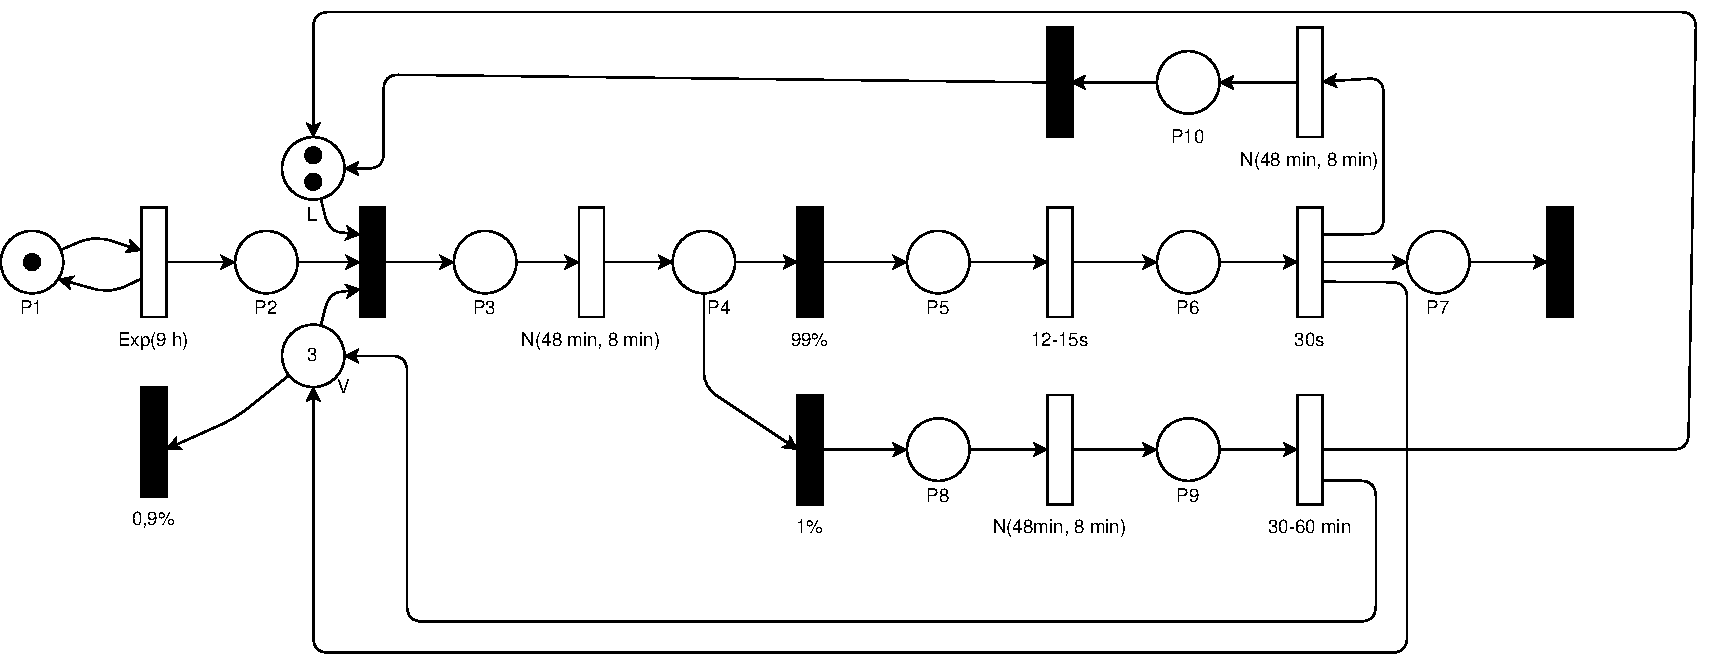
\includegraphics[scale=0.61, keepaspectratio]{fig/petri.pdf}
                \caption{Petriho síť}
                \label{fig:petri_nest}
            \end{figure}

            \begin{table}[H]
                \centering
                \begin{tabular}{ l l }
                    $P_1$ & Generování požadavků \\
                    $P_2$ & Fronta požadavků \\
                    $P_3$ & Přesun na bojiště \\
                    $P_4$ & Příprava na nabíjení \\
                    $P_5$ & Nabíjení \\
                    $P_6$ & Palba \\
                    $P_7$ & Odchod požadavků ze systému \\
                    $P_8$ & Přesun zpět do tábora (z~důvodu poruchy) \\
                    $P_9$ & Oprava houfnice \\
                    $P_{10}$ & Přesun zpět do tábora \\
                    $L$ & Linka houfnic \\
                    $V$ & Linka jednotek vojáků
                \end{tabular}
                \caption{Legenda k~Petriho síti}
                \label{tab:petri}
            \end{table}

    \section{Architektura simulačního modelu}
    \label{sec:architecture}

        Spuštěním simulačního modelu~\cite[snímek 44]{IMS_slides} se spustí simulační experiment se zadanými parametry.
        Parametry a jejich zadávání je popsáno v~kapitole~\ref{subsec:start}. Během simulačního experimentu jsou vypisovány všechny změny stavu,
        výpis každé změny stavu je doprovázen modelovým časem~\cite[snímek 21]{IMS_slides}. Modelový čas je vypisován v sekundách. Příkladem změny stavu může být např. to, že se autobus dostal do havárie. Nebo to, že sme na místo havárie poslali nový autobus, příjezd autobusu na zastávku, popřípadě na konečnou zastávku. Stavy jsou znázorněny v~Petriho síti,
        která reprezentuje konceptuální model v~kapitole~\ref{subsec:conceptual_model}.

        Pro účely simulace jsme si vybrali autobusovou linku č. 501, která jezdí z Ústředního hřbitova do Ořechova mimo dopravní špičku. Tomu odpovídají defaultní hodnoty našeho modelu, které vychází z jízdního řádu (např. jak daleko jsou od sebe jednotlivé autobusové zastávky).


        Simulační experiment v defaultním nastavení běží tak, aby co nejlépe popisoval autobusovou linku č. 501 mimo dopravní špičku.
        Experiment ve výchozím stavu běží tak, aby doba trvání experimentu odpovídala 6000 sekundám (1.66 hodinám) v~reálném čase~\cite[snímek 21]{IMS_slides}. Tato doba odpovídá době od výjezdu prvního autobusu až po tom, co poslední autobus přijede na konečnou zastávku, mimo dopravní špičku.
        Modelový čas~\cite[snímek 21]{IMS_slides} lze nastavit způsobem popsaným v~kapitole~\ref{subsec:start}. Jednotka modelového času je chápána jako
        sekunda v~reálném čase.
        Dále zde pracujeme se~šancí 5\%, že se autobus dostane do dopravní zácpy, ve které průměrně strávi 300 sekund (5 minut).\\ A s 0.00471\% šancí, že autobus zhavaruje. Obě proměnné jsou také nastavitelná, jelikož se můžou měnit na základě různých vnějších vlivů.

        \subsection{Mapování konceptuálního modelu do simulačního modelu}
        \label{subsec:mapping}

            Generování požadavků palby je reprezentováno třídou \texttt{Generátor}, která je implementována jako
            událost~\cite[snímek 169]{IMS_slides}. Proces přesunu na bojiště, nabíjení, palby a~návratu zpět, je 
            implementována třídou \texttt{Palba}. Dalším samostatným procesem je porucha (včetně přesunu zpět do tábora a~následné opravy),
            ta je reprezentována třídou \texttt{Porucha}. Proces dezerce jednotek vojáků je reprezentován třídou \texttt{Dezerce}.

        \subsection{Spouštění simulačního modelu}
        \label{subsec:start}

            Simulační experiment je možné spouštět s~parametry, pokud není parametr zadán, použije se výchozí hodnoty pro linku č.~501 popsané v kapitole \ref{sec:architecture}
            
            \begin{itemize}
                \item Parametr \texttt{-t} umožňuje nastavit modelový čas, jeho výchozí hodnota je 6000 sekund.
                \item Parametr \texttt{-a} umožňuje nastavit procento, s jakým se autobus dostane do havárky. Musí to být číslo v intervalu <0,1>.
                \item Parametr \texttt{-b} umožňuje nastavit počet autobusů, které operují na dané lince hromadné dopravy. Výchozí hodnota je 2.
                \item Parametr \texttt{-s} umožňuje nastavit počet autobusových zastávek na dané lince. výchozí hodnota je 7.
                \item Parametr \texttt{-l} umožňuje nastavit pruměrný čas mezi jednotlivými autobusovými zastávkami. Výchozí hodnota je 78 sekund (1.3 minuty).
                \item Parametr \texttt{-g} umožňuje nastavit interval, ve kterém vyjíždět jednotlivé autobusy.
                \item Parametr \texttt{-w} umožňuje nastavit čas, který průměrně autobus stráví v dopravní zácpě. Výchozí hodnota je 300s, což odpovídá 5 minutám.
                \item Parametr \texttt{-j} umožňuje měnit šanci, se kterou se autobus dostane do dopravní zácpy. Defaultně je nastavena na 0.00471. Parametr musí být číslo v intervalu <0,1>.
                \item Parametr \texttt{-c} umožňuje nastavit kapacitu cestujících autobusu. Výchozí hodnota je 75 cestujících.
            
            \item Parametr \texttt{-i} umožnuje nastavit pravou hranici intervalu <0,x> rovnoměrného rozložení, podle kterého se určuje počet cestujících na zastávce, kteří vstoupí do autobusu.
            \item Parametr \texttt{-o} umožnuje nastavit pravou hranici intervalu <0,y> rovnoměrného rozložení,podle kterého se určuje počet cestujících na zastávce, kteří vystoupí z~autobusu.
            \end{itemize}

            U~všech parametrů je vyžadováno kladné číslo.

            Program (s~výchozími hodnotami) je možné spustit příkazem \texttt{make run}.

    \section{Podstata simulačních experimentů a~jejich průběh}
    \label{sec:simulation}

        Cílem experimentů bylo pozorování chování modelu.
        Účelem bylo zjistit, na základě chování modelu, optimální jízdní řád na danou linku hromadné dopravy (v našem případě linka č. 501). Optimální jízdní řád zjišťujeme na základě spokojenosti cestujících. Pokud cestující přijel včas do cílové zastávky, předpokládáme, že je spokojen. Pokud přijel se zpožděním, předpokládáme, že nebyl spokojen. Výstupem pak je průměrná spokojenost cestujícího v daném autobusu, která může být buď kladná, nebo záporná.

        \subsection{Postup experimentování}
        \label{subsec:experiments_methods}

            Samotný experiment byl spouštěn s danými parametry, které jsme zanesli do tabulky. Pokud některé parametry nejsou v tabulce zaneseny, počítáme s jejich defaultní hodnotou. Poslední položka tabulky je vždy spokojenost cestujících, která nám říká, jestli byl průměrně cestující s jízdou spokojen, či nikoliv. Pokud byl průměrně cestující spokojen, můžeme říci, že jízdní řád je sestaven správně a celkový počet autobusů na lince je v pořádku. Pokud je spokojenost cestujících podprůměrná, musíme se zamyslet, kde nastala chyba. U každého experimentu je také screenshot s výstupem našeho nástroje.
            Pokud by byla modelována jiná linka, pomocí parametrů lze nastavit všechny potřebné proměnné. Náš model je tímto ve svém oboru zajímavý, jelikož se dá použít na jakoukoliv linku hromadné dopravy.
        \newpage
        \subsection{Experimenty}
        \label{subsec:experiments}

            Každý experiment je spuštěn s danými parametry, má úvod a závěr. Nachází se u~něj výpis spokojenosti cestujících a screenshost z výstupu simulace.

            \subsubsection{Experiment 1}
            \label{subsubsec:experiment1}

                Cílem tohoto experimentu je ověření
                toho, jestli jízdní řád linky č. 501 \cite{Jizdni_rad} funguje správně v časy mimo dopravní špičku při nízkém vytížení cestujícími. Jsou použity výchozí hodnoty.

                \begin{table}[H]
                    \centering
                    \resizebox{\textwidth}{!}{
                    \begin{tabular}{ | c | c | c | c | c | c | c | c| }
                        \hline
                         Celkový čas (s) & Počet autobusů &  Počet zastávek & Průměrný čas mezi zastávkami & Šance na dopravní zácpu & Čas v dopravní zácpě (s) & Šance na havárii & Spokojenost\\
                        \hline
                        \hline
                        6000 & 2 & 7 & 78 & 5\% & 300 & 0.00471\% & \textcolor[rgb]{0,0.5,0}{Kladná}\\
                        \hline
                    \end{tabular}
                    }
                    \caption{Výsledek experimentu 1}
                    \label{tab:experiment1}
                \end{table}

                Na obrázku \ref{fig:experiment1} vidíme výstup naší simulace a můžeme vidět, že když neuvažujeme dopravní spičku, jízdní řád autobusové linky č. 501 je vytvořen správně. Lidé jsou spokojeni a průměrný čas v dopravních zácpách je velmi malý. Takže autobus přijel se zanedbatelním zpožděním.

                \begin{figure}[H]
                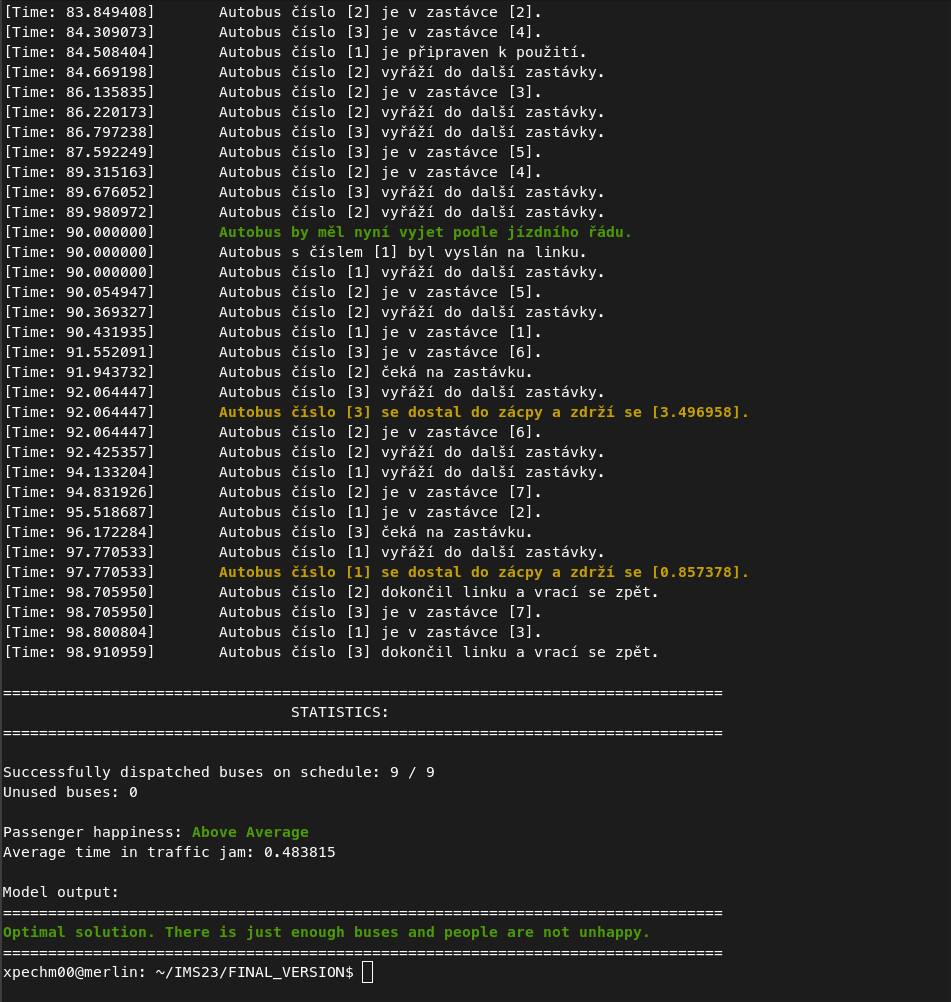
\includegraphics[scale=0.45, keepaspectratio]{fig/ims_bus1.png}
                \caption{Experiment 1 - mimo dopravní špičku}
                \label{fig:experiment1}
            \end{figure}
        \newpage
            \subsubsection{Experiment 2}
            \label{subsubsec:experiment2}

                V~tomto experimentu se pokusíme zjistit, jak se námi vybraná autobusová linka č. 501 chová, v dopravní špičce, kdy je větší šance dostat se do zácpy a nastupuje více lidí, než obvykle. 

                \begin{table}[H]
                    \centering
                    \resizebox{\textwidth}{!}{
                    \begin{tabular}{ | c | c | c | c | c | c| c |}
                        \hline
                        Šance na dopravní zácpu & \footnote{Rovnoměrné rozložení, které udává počet cestujících nastupujících do autobusu, je dáno tímto intervalem}Interval nástupu & \footnote{Rovnoměrné rozložení, které udává počet cestujících vystupujících z autobusu, je dáno tímto intervalem}Interval výstupu & Doba strávená v zácpe (s) & Průměrný čas mezi zastávkami (s)& Šance na havárii & Spokojenost \\
                        \hline
                        \hline
                        14\% & <0,20> &<0,2>& 1020 & 85 & 1\%  & \textcolor{red}{Podprůměrná}\\
                        \hline
                    \end{tabular}
                    }
                    \caption{Parametry experimentu 2}
                    \label{tab:experiment2}
                \end{table}

                Z~obrázku~\ref{fig:experiment2} vidíme, že pokud se jedná o dopravní špičku, tak jsou cestující nespokojení. Strávili spoustu času v dopravní zácpě a přijeli pozdě. V tomto případě by možné řešení byl zvýšit počet autobusů na lince v době dopravních špiček a změnšit interval, ve kterém autobusy po sobě vyjíždí.

                \begin{figure}[H]
                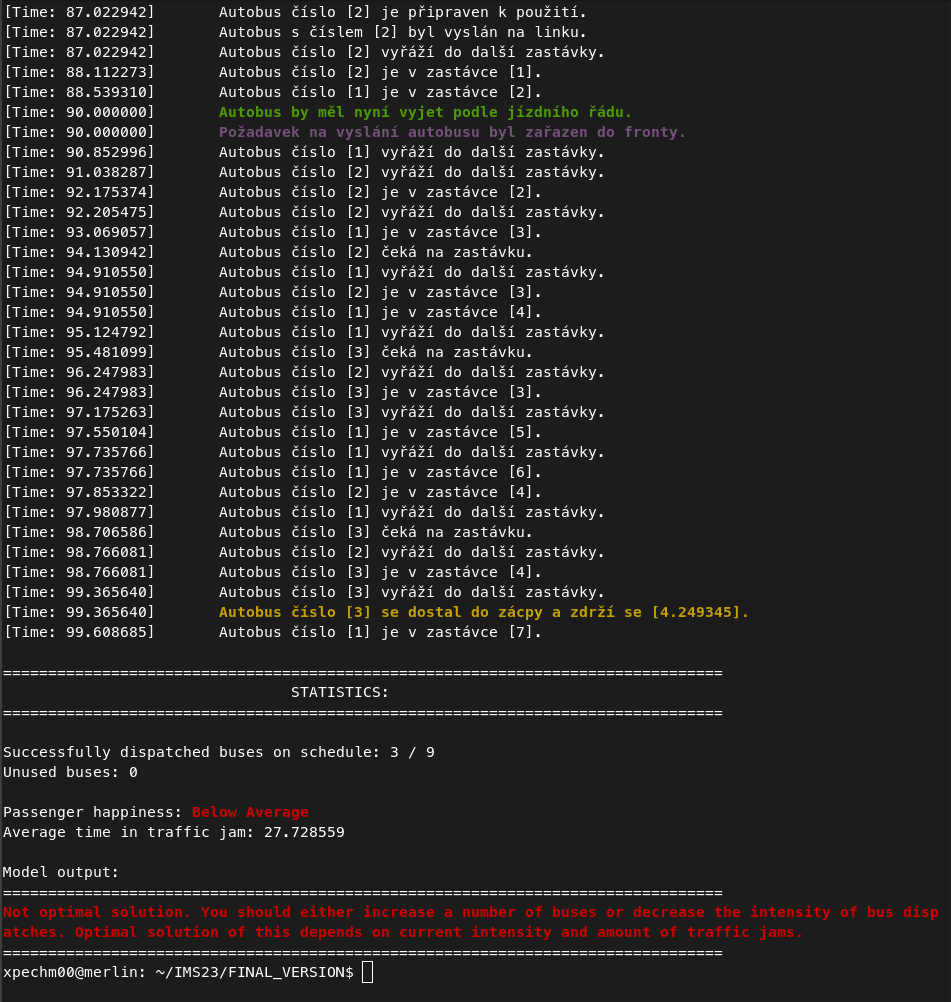
\includegraphics[scale=0.48, keepaspectratio]{fig/ims_bus2.png}
                \caption{Výsledek experimentu 2 - dopravní špička}
                \label{fig:experiment2}
            \end{figure}
    \newpage
            \subsubsection{Experiment 3}
            \label{subsubsec:experiment3}

                V jízdním řádu \cite{Jizdni_rad} si můžeme všimnout, že občas autobus jezdí "zkrácenou linku". Neboli nevyjíždí z Ústředního hřbitova, ale až z druhé zastávky, z Ořechovské. Důvodem je, že mezi první a druhou zastávkou bývá v dopravní špičce velká pravděpodobnost toho, že se autobus dostane do zácpy, a že ta zácpa bude trvat déle než je únosné. Proto zkusíme otestovat, jaký bude výstup naší simulace, když nastavíme parametry, které budou představovat zkrácenou linku v dopravní špičce.
                

                \begin{table}[H]
                    \centering
                     \resizebox{\textwidth}{!}{
                    \begin{tabular}{ | c | c | c | c | c | c | c |}
                        \hline
                        Počet zastávek & \footnote{Rovnoměrné rozložení, které udává počet cestujících nastupujících do autobusu, je dáno tímto intervalem}Interval nástupu& \footnote{Rovnoměrné rozložení, které udává počet cestujících vystupujících z autobusu, je dáno tímto intervalem} Interval výstupu & Průměrný čas v zácpě (s)& Průměrný čas mezi zastávkami (s) & Šance na havárii &spokojenost\\
                        \hline
                        \hline
                        6 & 20 & 2 & 500 & 85 &1\% & \textcolor[rgb]{0,0.5,0}{Nadprůměrná}\\
                        \hline
                    \end{tabular}
                    }
                    \caption{Parametry experimentu 3}
                    \label{tab:experiment3}
                \end{table}

            

                Na obrázku \ref{fig:experiment3} můžeme vidět, že zkrácená linka funguje i v dopravní špičce, takže dává smysl ji v jízdním řádu zachovat tak, jak je.

                \begin{figure}[H]
                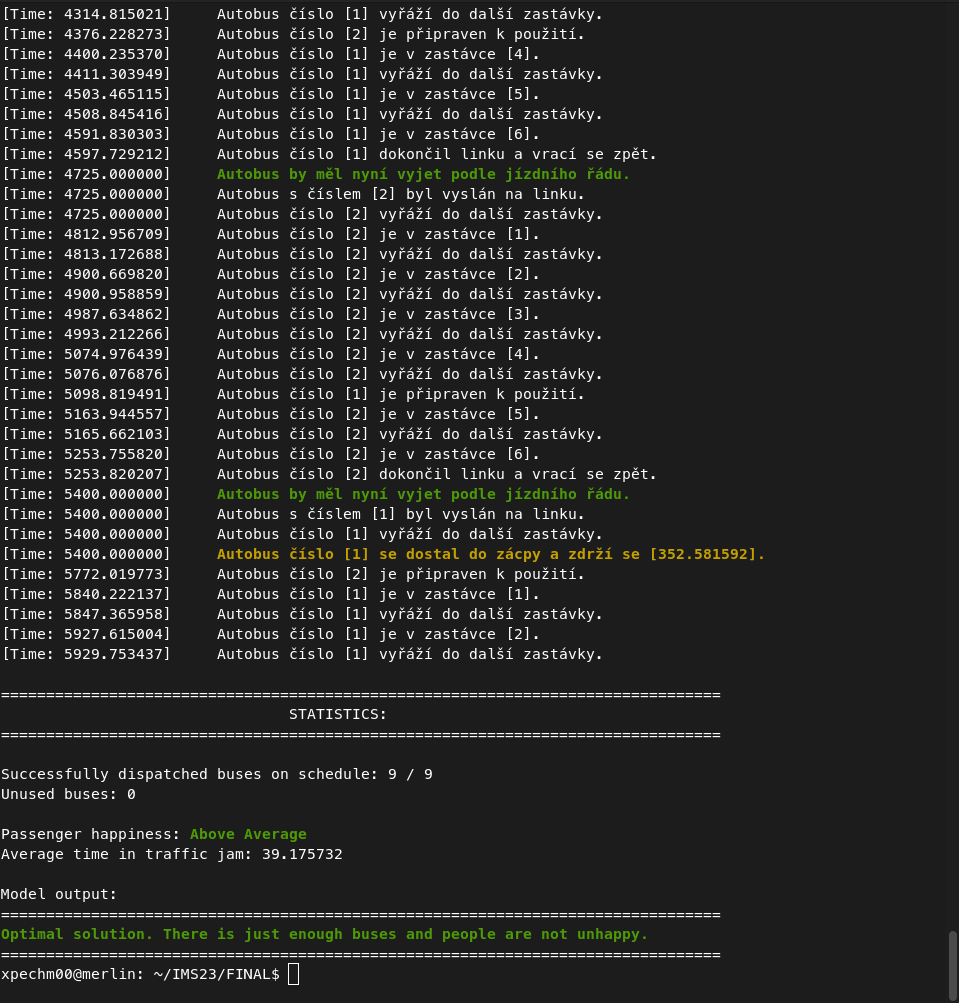
\includegraphics[scale=0.48, keepaspectratio]{fig/ims_bus3.png}
                \caption{Výsledek experimentu 3 - zkrácená linka v dopravní špičce}
                \label{fig:experiment3}
            \end{figure}
            \newpage
            \subsubsection{Experiment 4}
            \label{subsubsec:experiment4}
                V~tomto experimentu budeme zkoumat klasickou nezkrácenou linku mimo dopravní špičku


                V~tomto experimentu budeme vycházet z~hodnot a~výsledků experimentu 3 v~kapitole~\ref{subsubsec:experiment3} a~vyzkoušíme,
                zda jsou dobře využitelné i~v~delším časovém intervalu, v~tomto případě 7 dní (10080 minut).

                \begin{table}[H]
                    \centering
                    \begin{tabular}{ | c | c | c | c | c | }
                        \hline
                        Intenzita požadavků [min] & Celkový čas [min] & Bez čekání & S~čekáním & Celkem \\
                        \hline
                        \hline
                        130 & 10080 & 65 & 12 & 77 \\
                        \hline
                    \end{tabular}
                    \caption{Výsledky experimentu 4}
                    \label{tab:experiment4}
                \end{table}

                Z~výsledků je patrné, že počet požadavků, které musely na svoji obsluhu čekat, narostl,
                stále však byla většina požadavků obsloužena bez čekání.

                 \begin{figure}[H]
                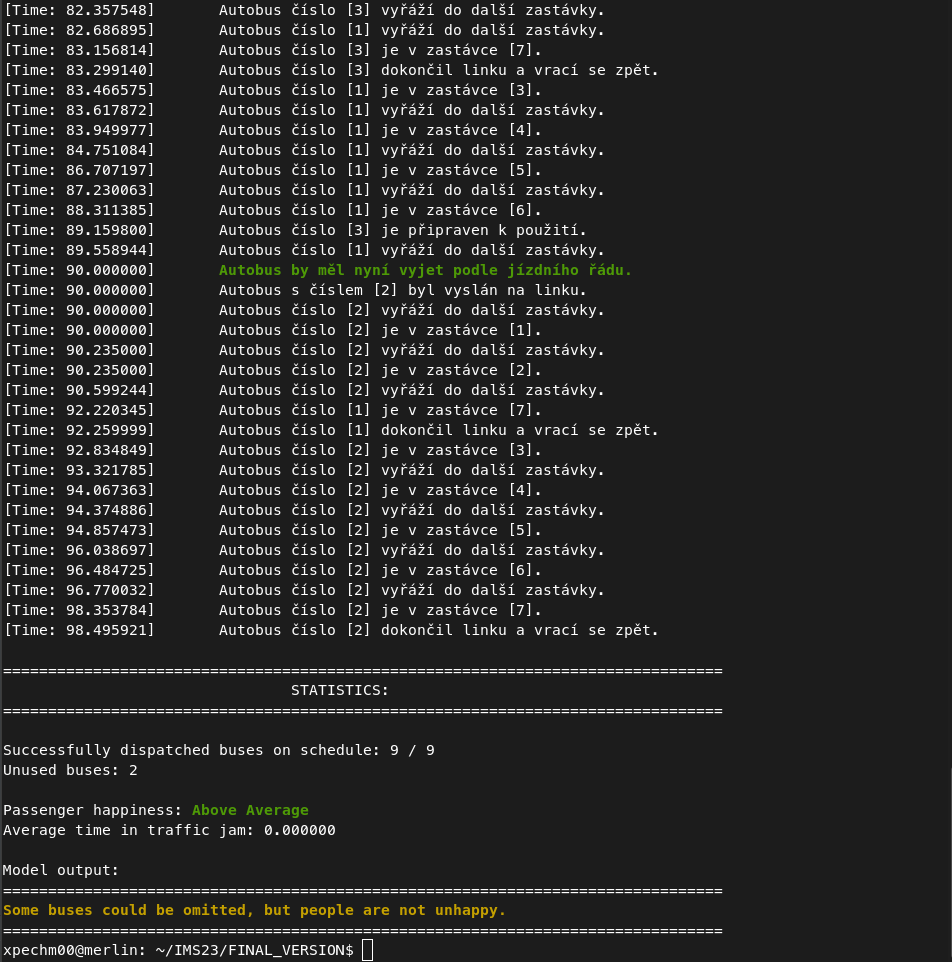
\includegraphics[scale=0.37, keepaspectratio]{fig/ims_bus4.png}
                \caption{Výsledek experimentu  - zkrácená linka v dopravní špičce}
                \label{fig:experiment4}
                    \end{figure}

            \newpage
            \subsubsection{Experiment 5}
            \label{subsubsec:experiment5}

                Cílem posledního experimentu bylo vyzkoušet, jak by autobusová linka fungovala, kdyby na ní jezdil jen 1 autobus.
    
                \begin{table}[H]
                    \centering
                    \begin{tabular}{ | c | c |}
                        \hline
                        Počet autobusů & Spokojenost\\
                        \hline
                        \hline
                        1 & \textcolor{red}{Podprůměrná} \\
                        \hline
                    \end{tabular}
                    \caption{Parametry experimentu 5}
                    \label{tab:experiment5}
                \end{table}

            Jak můžeme vidět na obrázku \ref{fig:experiment5}, pokud by jezdil jen jeden autobus v podmínkách dané klasickou nezkrácenou linkou mimo dopravní špičku, spokojenost cestujících by byla negativní. Bud bychom museli zvýšit počet autobusů a nebo snížit frekvenci, s jakou autobusy jezdí (např. autobus by jezdil jen každé 3h).
                
                \begin{figure}[H]
                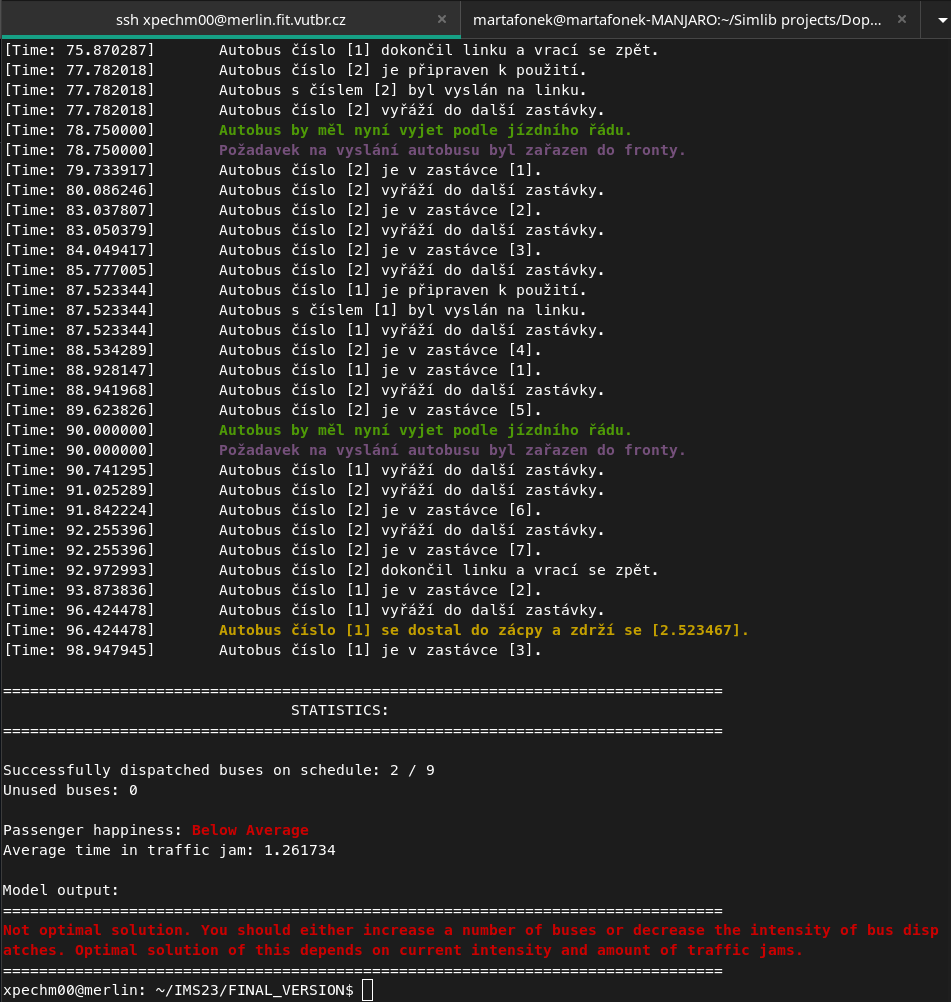
\includegraphics[scale=0.37, keepaspectratio]{fig/ims_bus5.png}
                \caption{Výsledek experimentu 5 - nízký počet autobusů}
                \label{fig:experiment5}
            \end{figure}

        \subsection{Závěry experimentů}
        \label{subsec:experiments_summary}

            Bylo provedeno 5 experimentů s~různými parametry. V prvním experimentu jsme ověřili, že mimo dopravní špičku funguje jízdní řád autobusové linky č. 501 optimálně. V dalších experimentech jsme např. testovali, jak se autobusová linka chová, když je dopravní spička, tedy cestuje více cestujících a je větší šance na to, že se autobus dostane do zácpy. Došli jsme k závěru, že pokud bychom měli normální jízdní řád, v době dopravních špiček by byl značně nevyhovující. Dále jsme otestovali, jestli momentální řešení Českých drah funguje. Tedy zkusili jsme simulaci spustit nad zkrácenou linkou, která nevyjíždí z první zastávky, ale až z druhé. Ukázalo se, že aktuální řešení funguje. Zkusili jsme také simulaci spustit nad jednoznačně malým množstvím autobusů u linky a ukázalo se, že pokud bychom měli jen jeden autobus na tuto linku, momentální stav jízdního řádu by byl nevyhovující a musel by se změnit. Pokud bychom si nemohli dovolit přidat další autobus na linku, museli bychom zvětšit prodlevu mezi jednotlivými cesty autobusu.
            
            
            Experimenty lze považovat s~dostatečnou věrohodností za správný zdroj informací, protože jich bylo provedeno několik a odpovídají již existujícímu jízdnímu řádu dané linky.
\newpage
    \section{Shrnutí simulačních experimentů a~závěr}
    \label{sec:summary}
            V~rámci našich experimentů jsme ověřili, že momentální jízdní řád autobusové linky č. 501 je správně vymyšlen a dobře řeší problematiku dopravních špiček.

            Za validaci výsledků můžeme považovat to, že naše výstupy korespondují s jízdním řádem.

            Vytvořili jsme nástroj, který je schopen pomáhat s tvorbou ideálních jízdních řádů. Nástroj byl implementován v jazyce C++ a využívá knihovnu SIMLIB. Umožňuje spouštět simulační experimenty s různými parametry, takže se dá využít nad libovolnou linkou hromadné dopravy. Vstupem jsou tedy parametry linky hromadné dopravy (popsáno v sekci \ref{subsec:start}) a výstupem je spokojenost cestujících, podle které můžeme parametry iterativně upravovat, abychom dostali ideální jízdní řád pro danou linku. 

            Nástroj by se mohl využívat přímo provozovatelem autobusů. Za předpokladu, že by měl svá přesnější data (např. ohledně počtu cestujících na jednotlivých zastávkách), mohl by velmi efektivně zoptimalizovat své jízdní řády a počty autobusů na jednotlivých linkách. Výsledkem by mělo být, že více cestujících bude spokojených se službou hromadné dopravy.
            


    \newpage

    \renewcommand{\refname}{Použitá literatura}
    \bibliographystyle{czechiso}
    \bibliography{documentation}

\end{document}
